\documentclass{article}
\usepackage{graphicx} % This lets you include figures
\usepackage{subcaption} % This lets you include sib figures

\begin{document}

This document will note and explain the changes done to the LIMB project during the summer of 2026

\section{Mechanical}

\subsection{Shoulder Up-Down Worm \& Worm gear}

The original worm broke. 
\begin{figure}[h]
    \begin{subfigure}{.5\textwidth}
        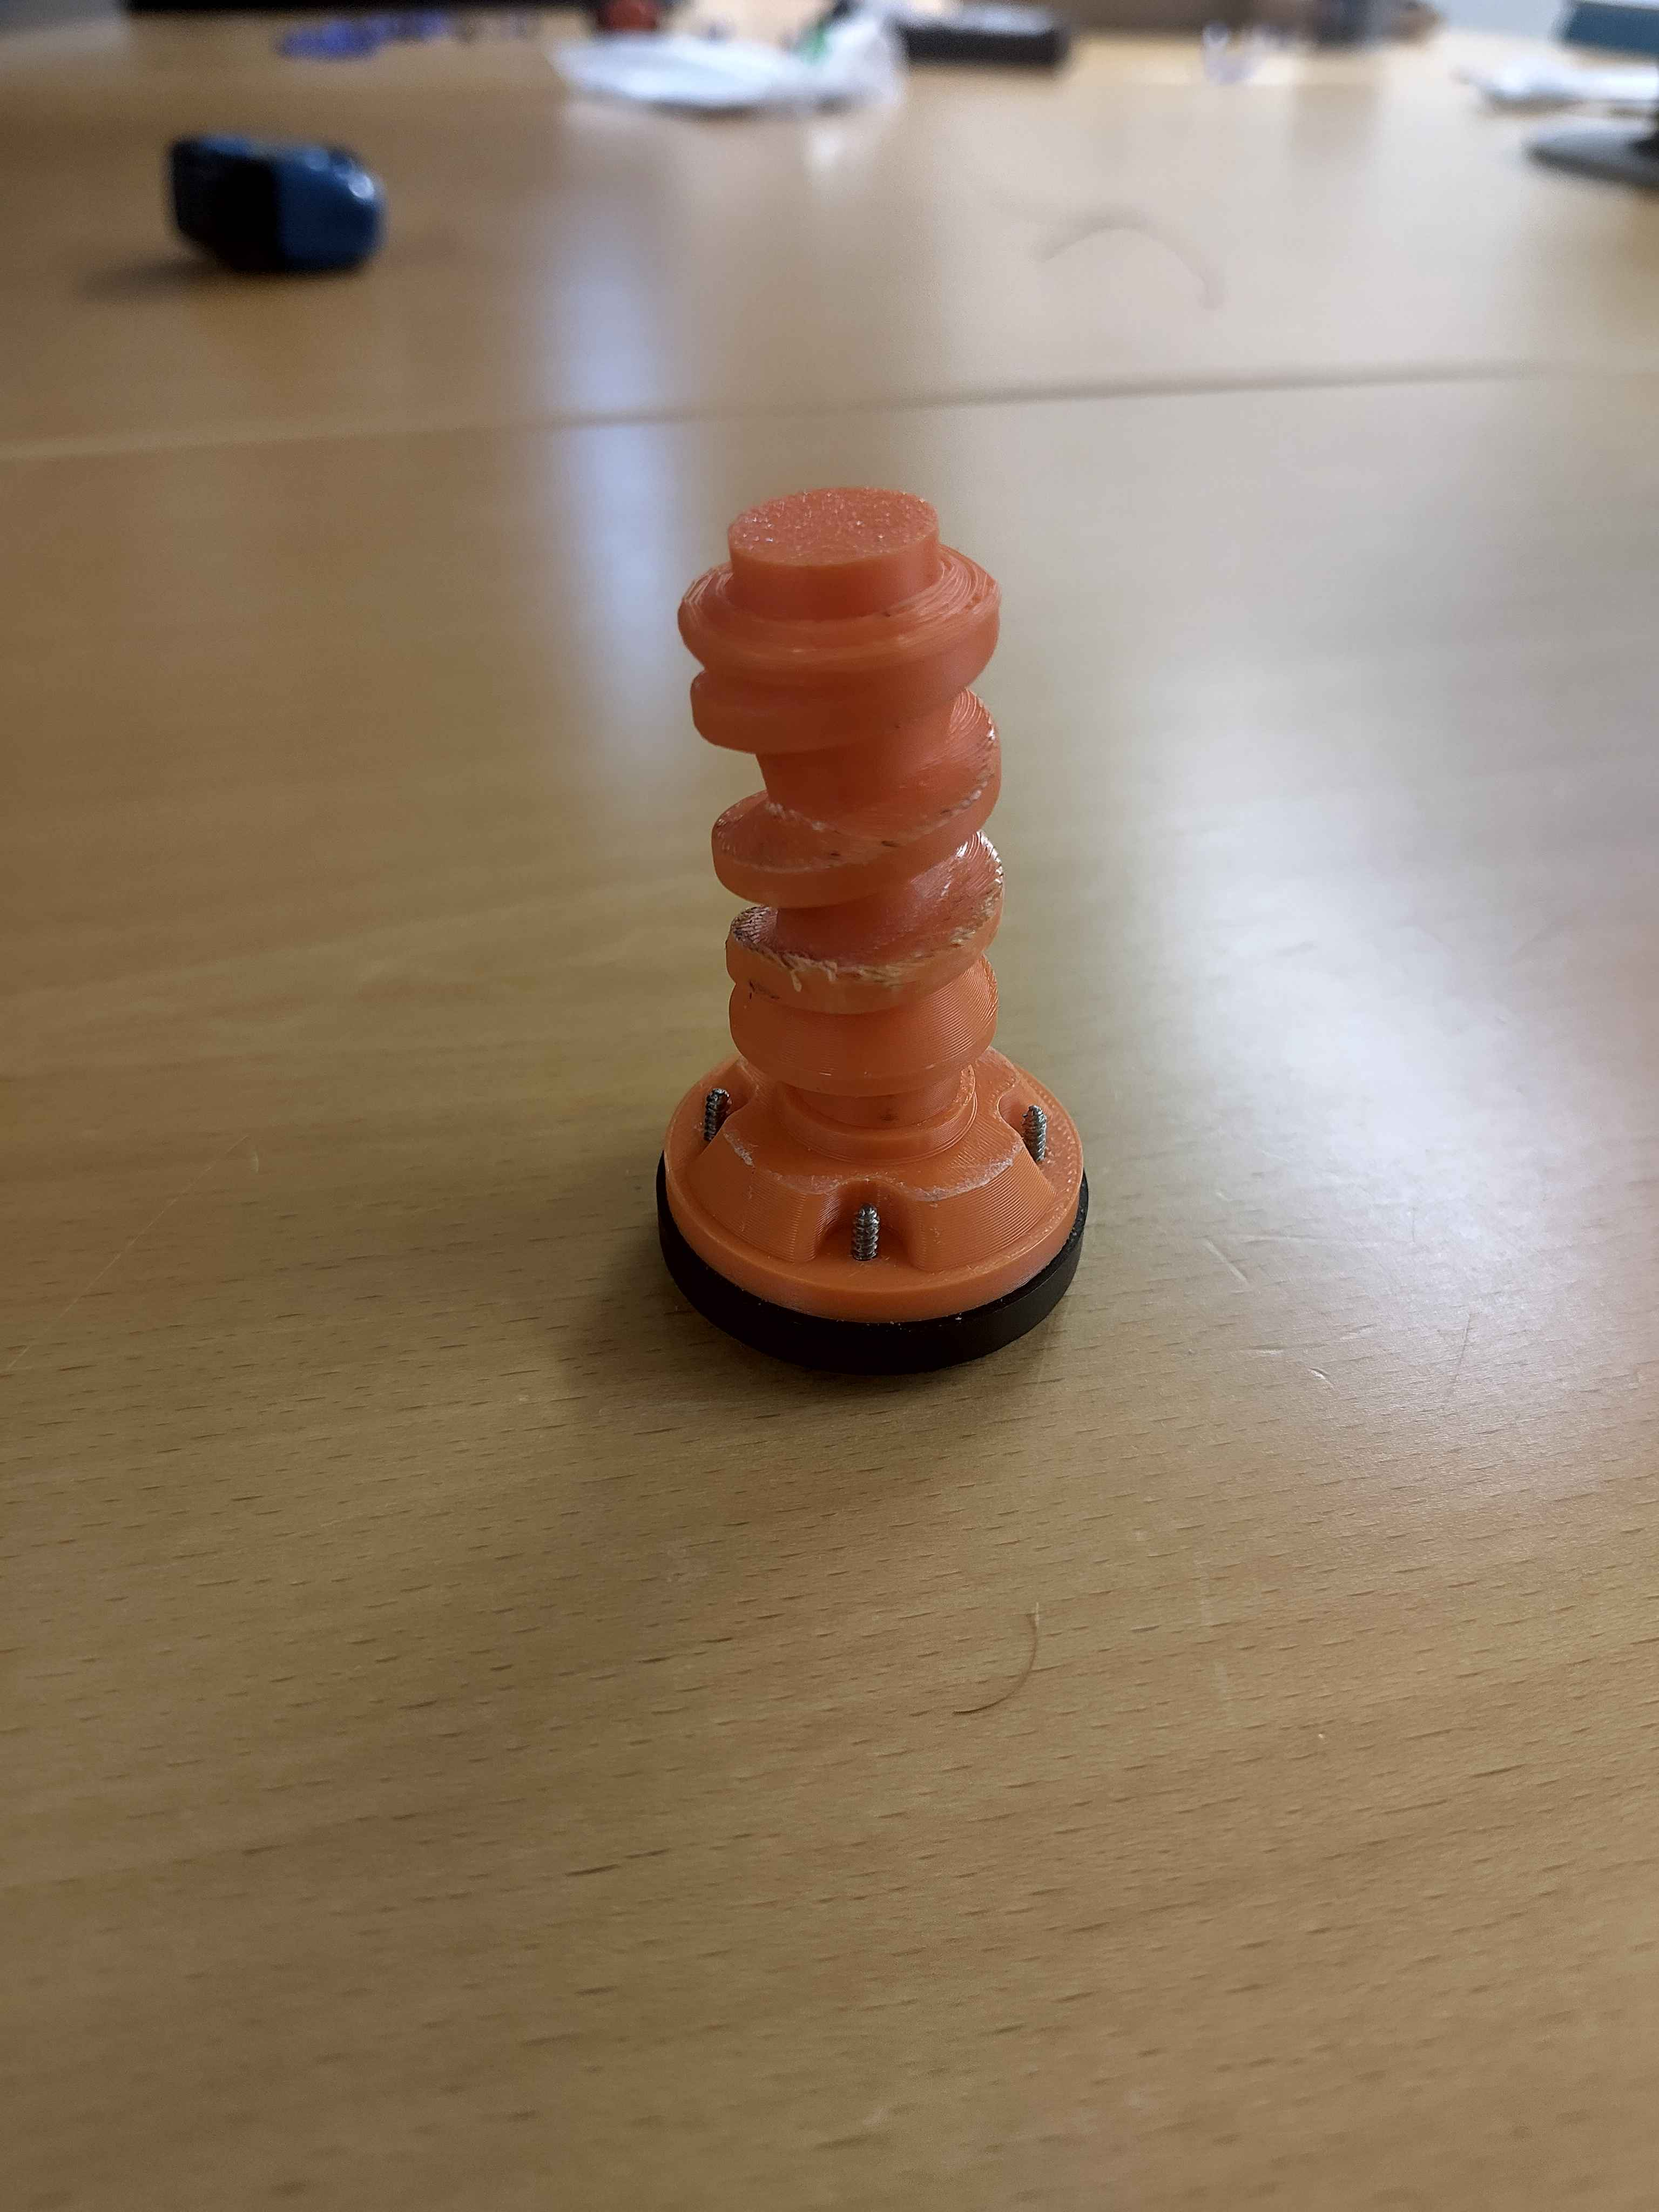
\includegraphics[width=.8\linewidth]{Media/Worm_Bent.jpg}
    \end{subfigure}
    \begin{subfigure}{.5\textwidth}
        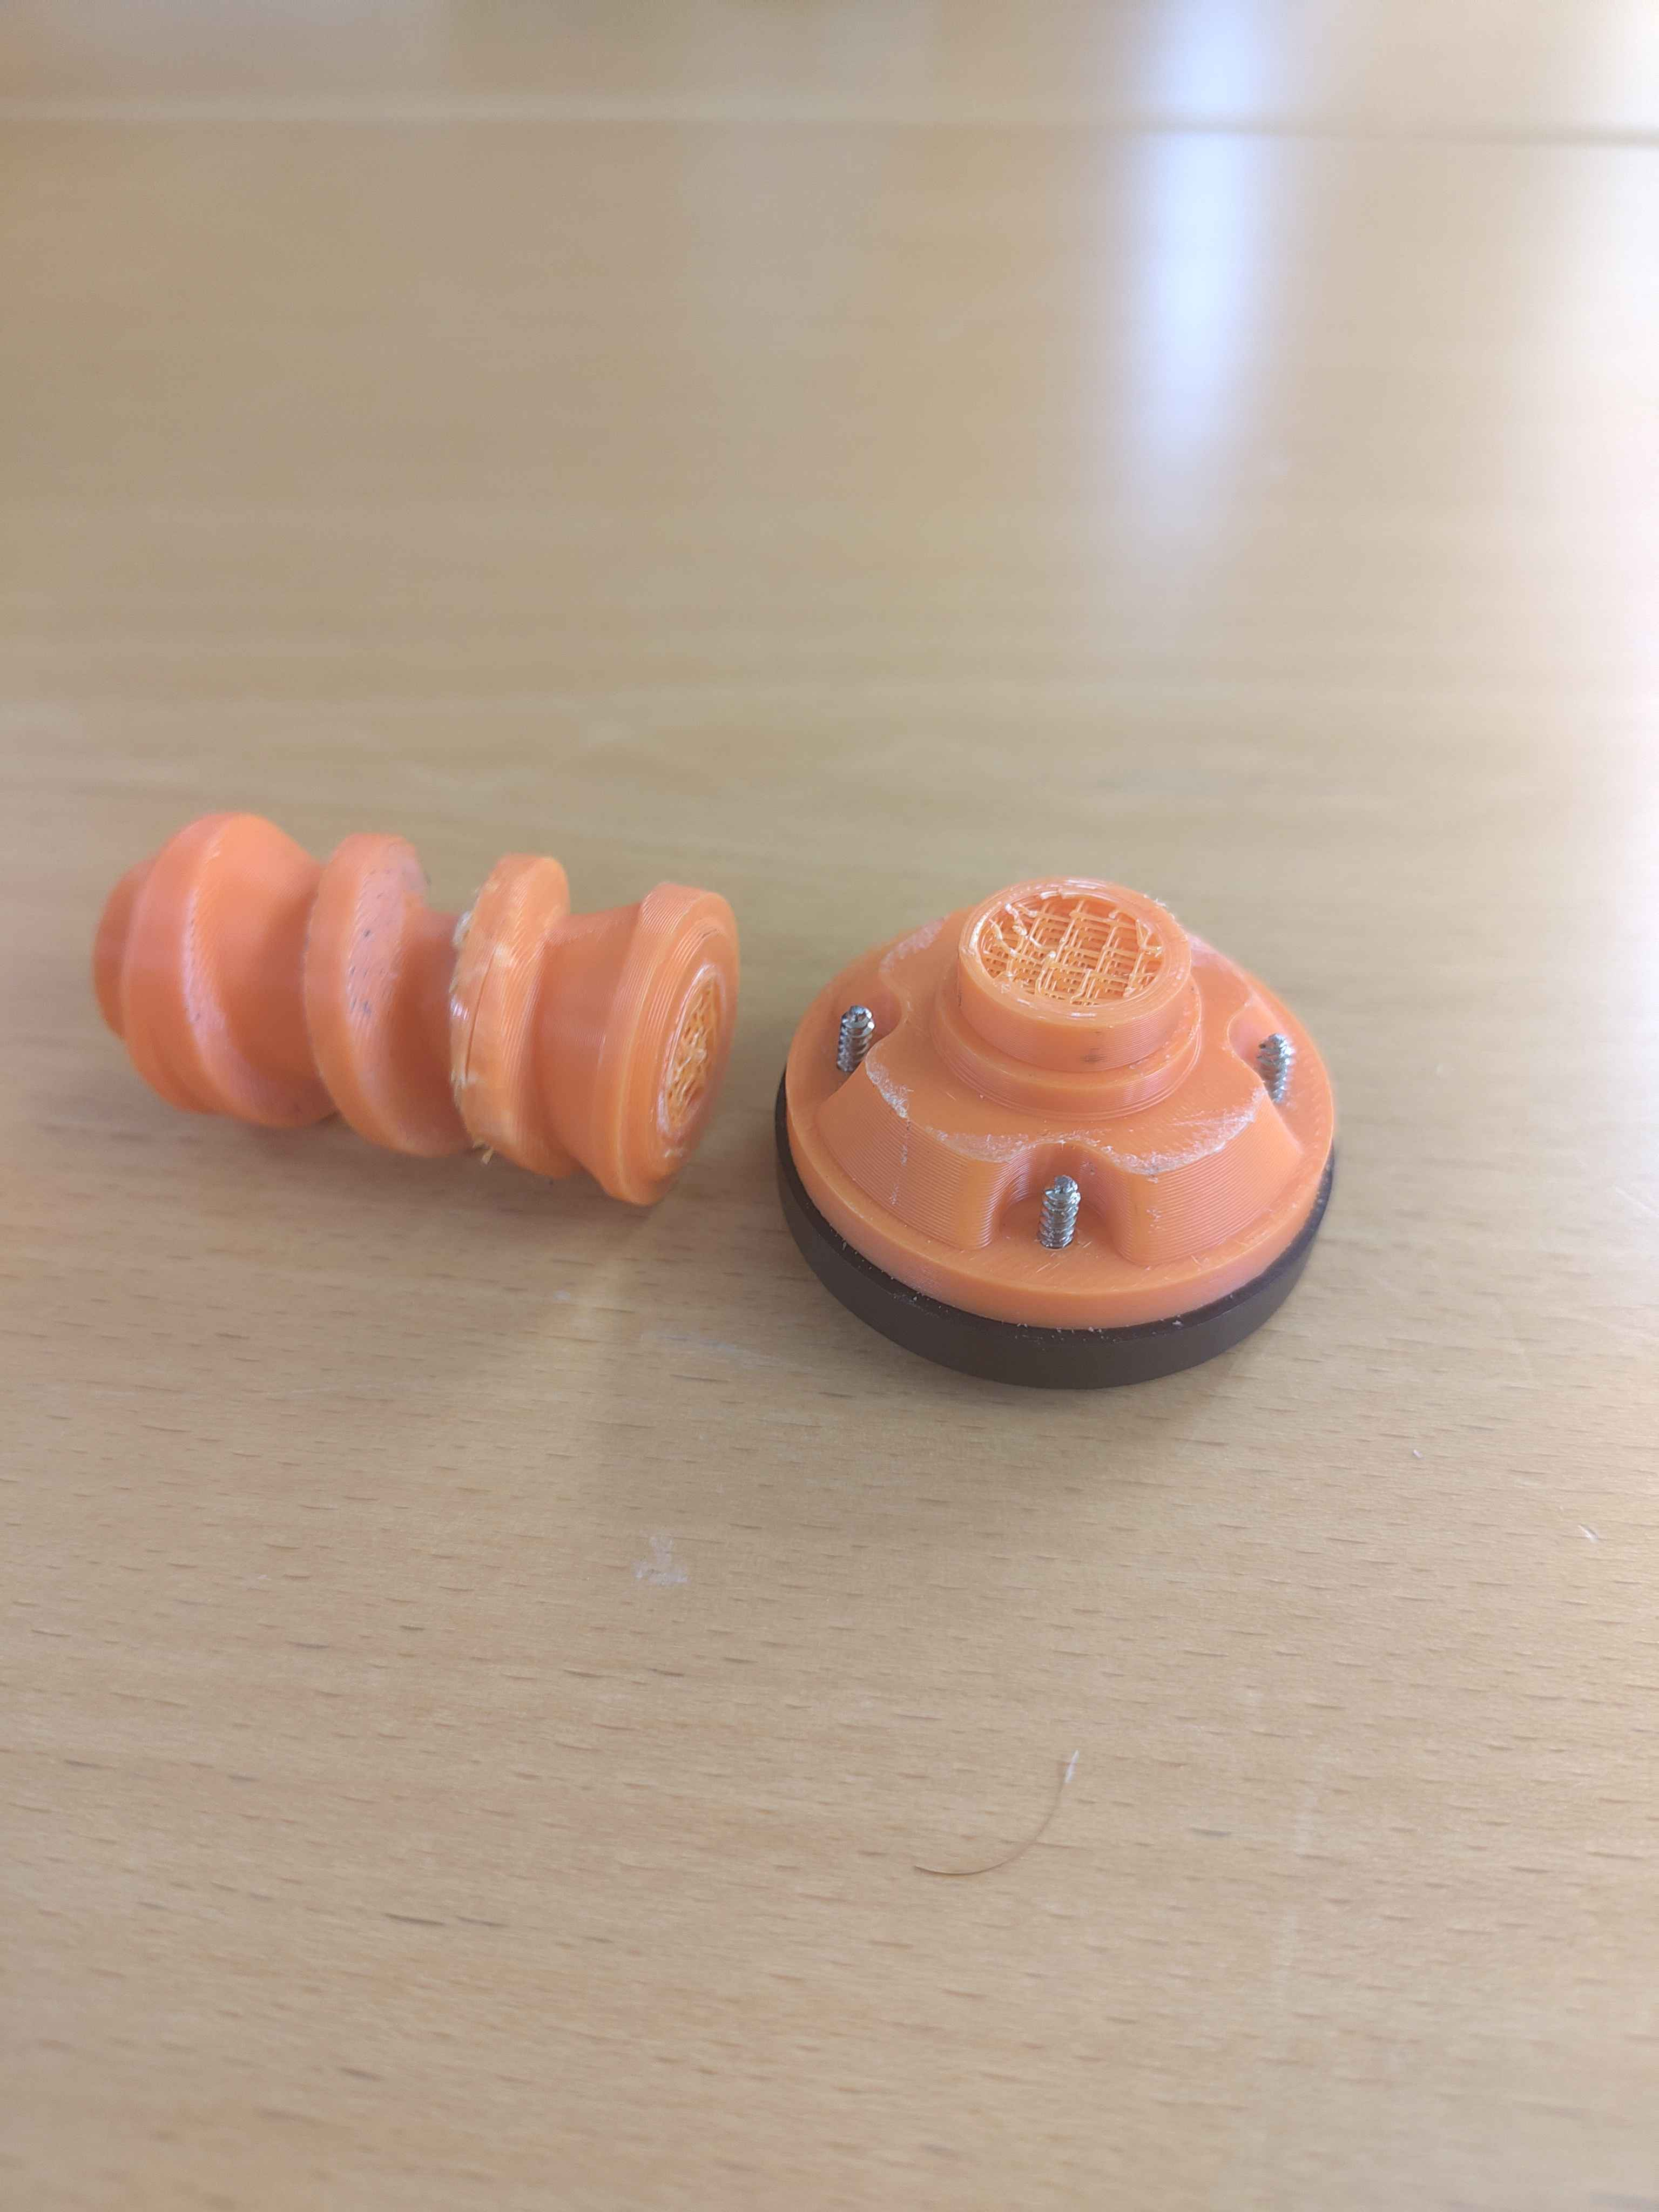
\includegraphics[width=.8\linewidth]{Media/Worm_Broke.jpg}
    \end{subfigure}
\end{figure}

A new worm was printed out of carbonfibre. It also broke along with the motor driving it.

\begin{figure}[h]
    \begin{subfigure}{.5\textwidth}
        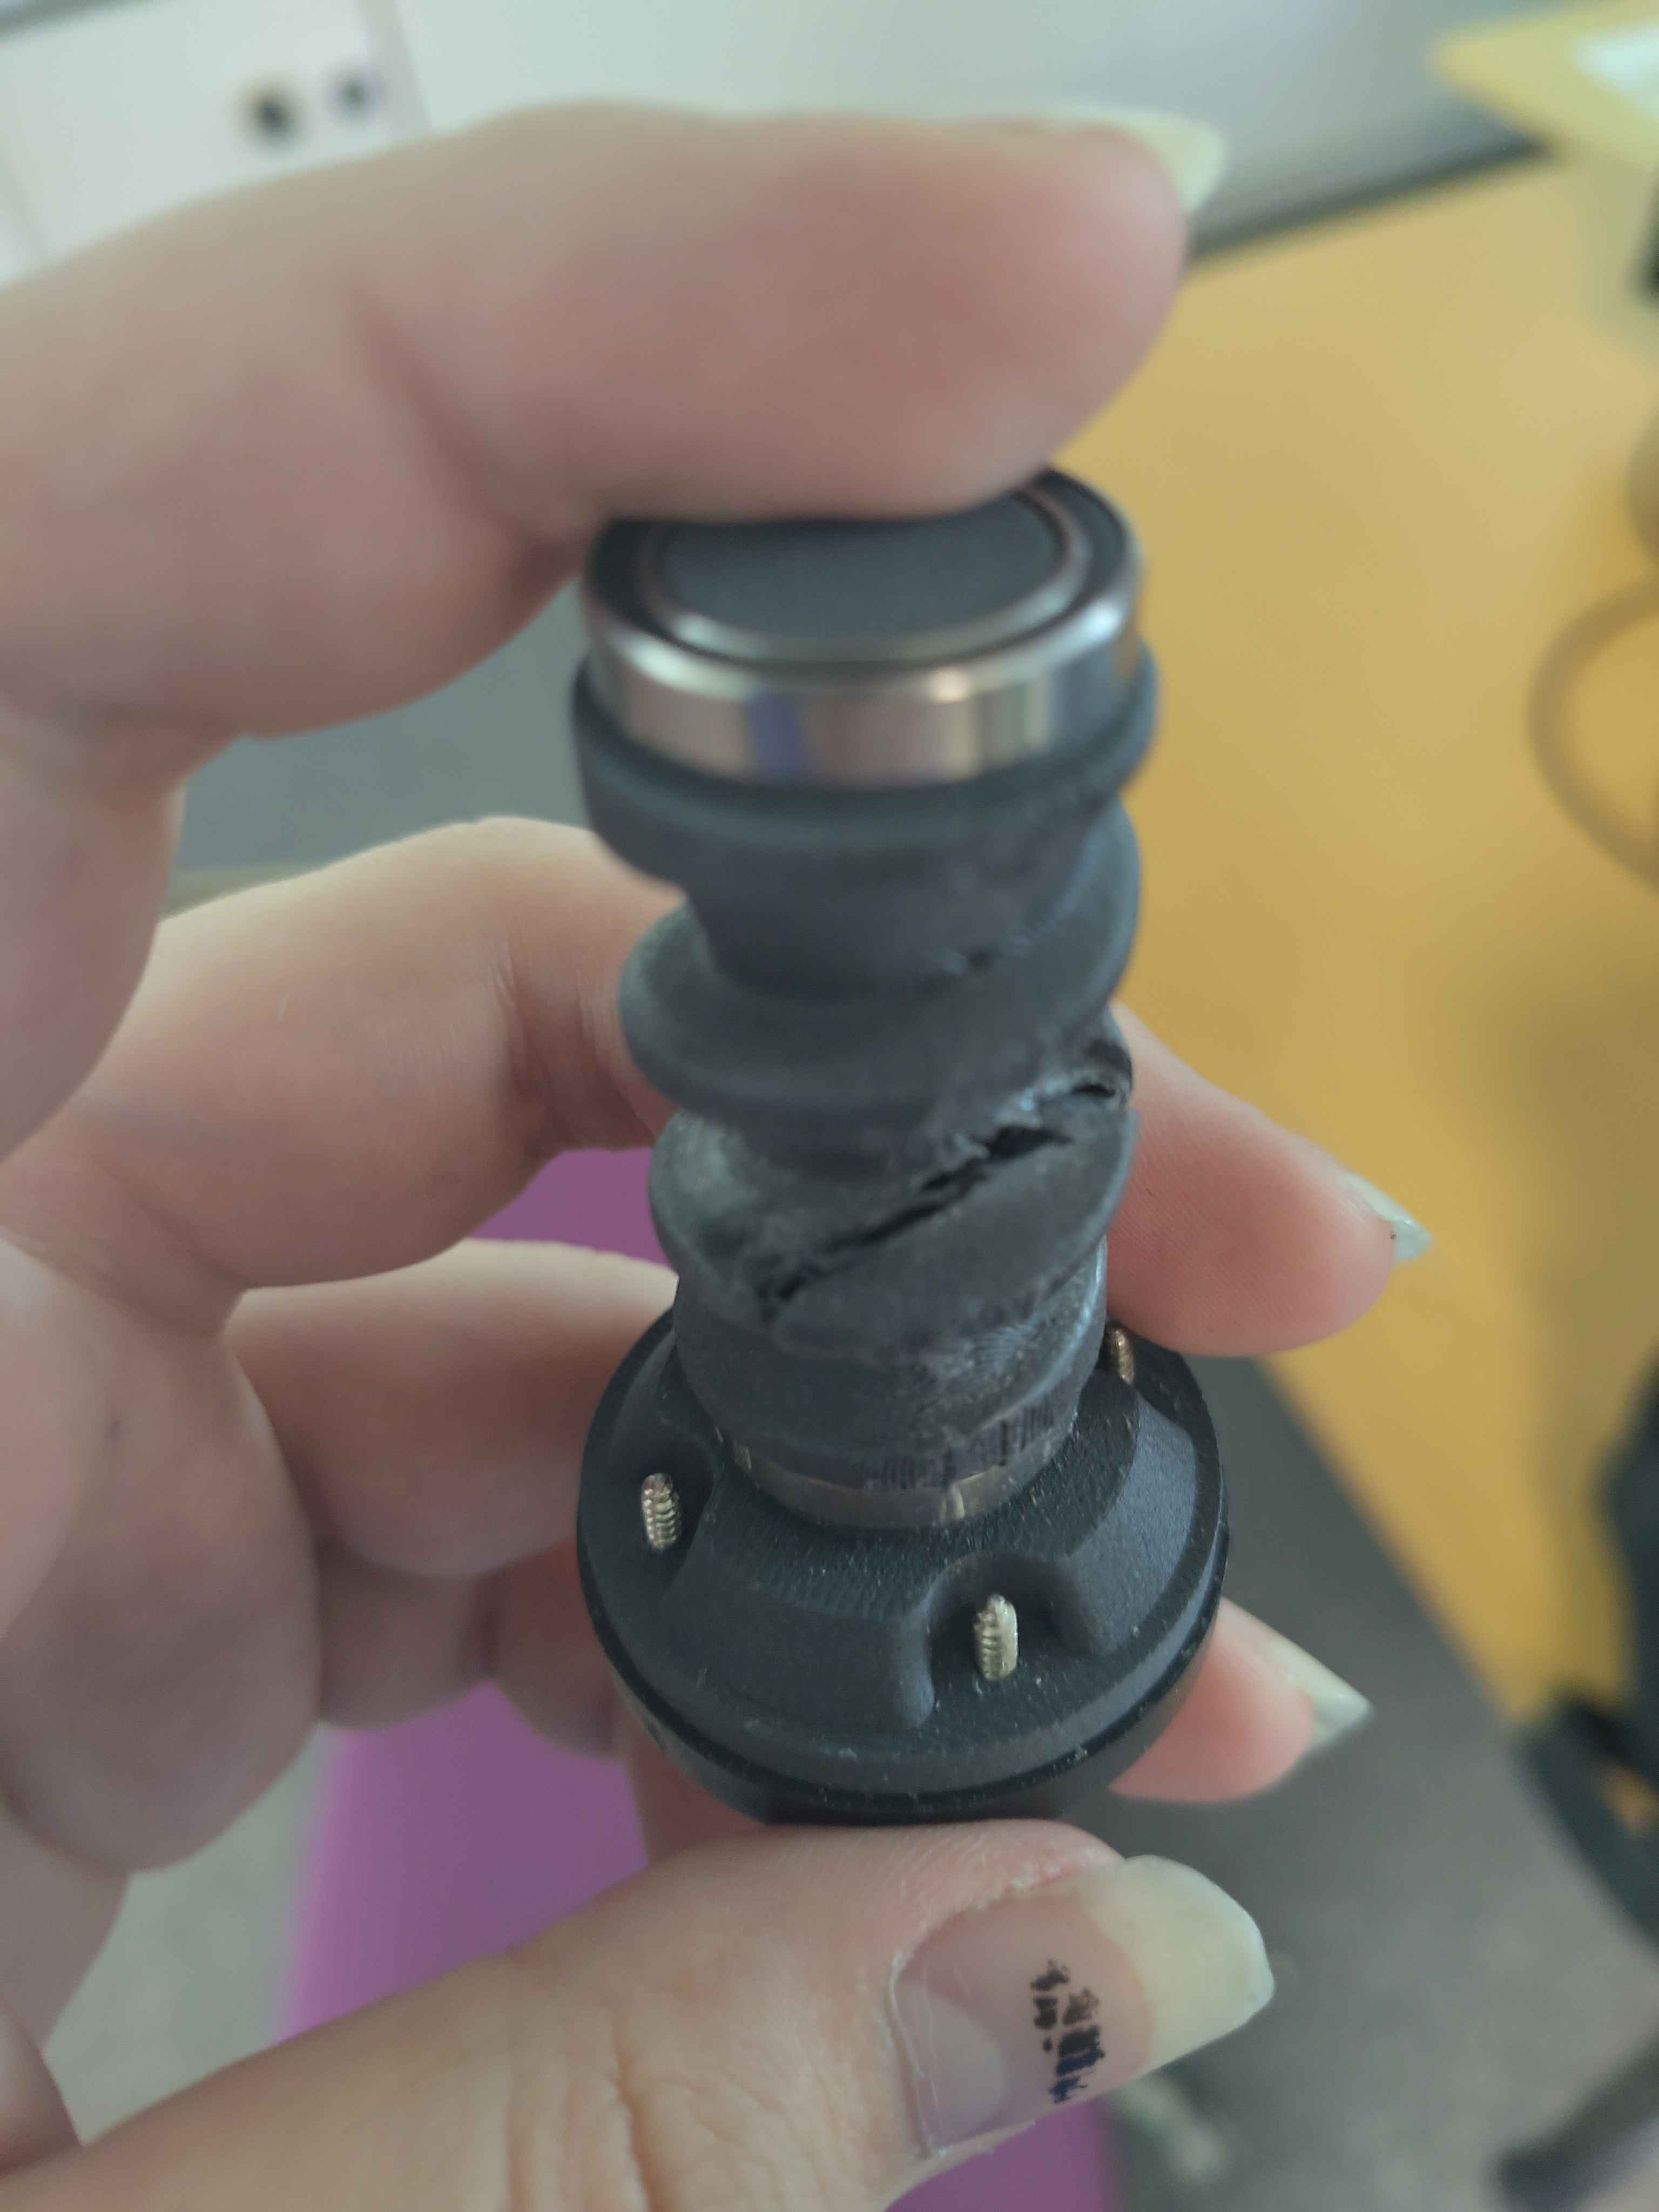
\includegraphics[width=.8\linewidth]{Media/Carbon_Worm_Broke.jpg}
    \end{subfigure}
    \begin{subfigure}{.5\textwidth}
        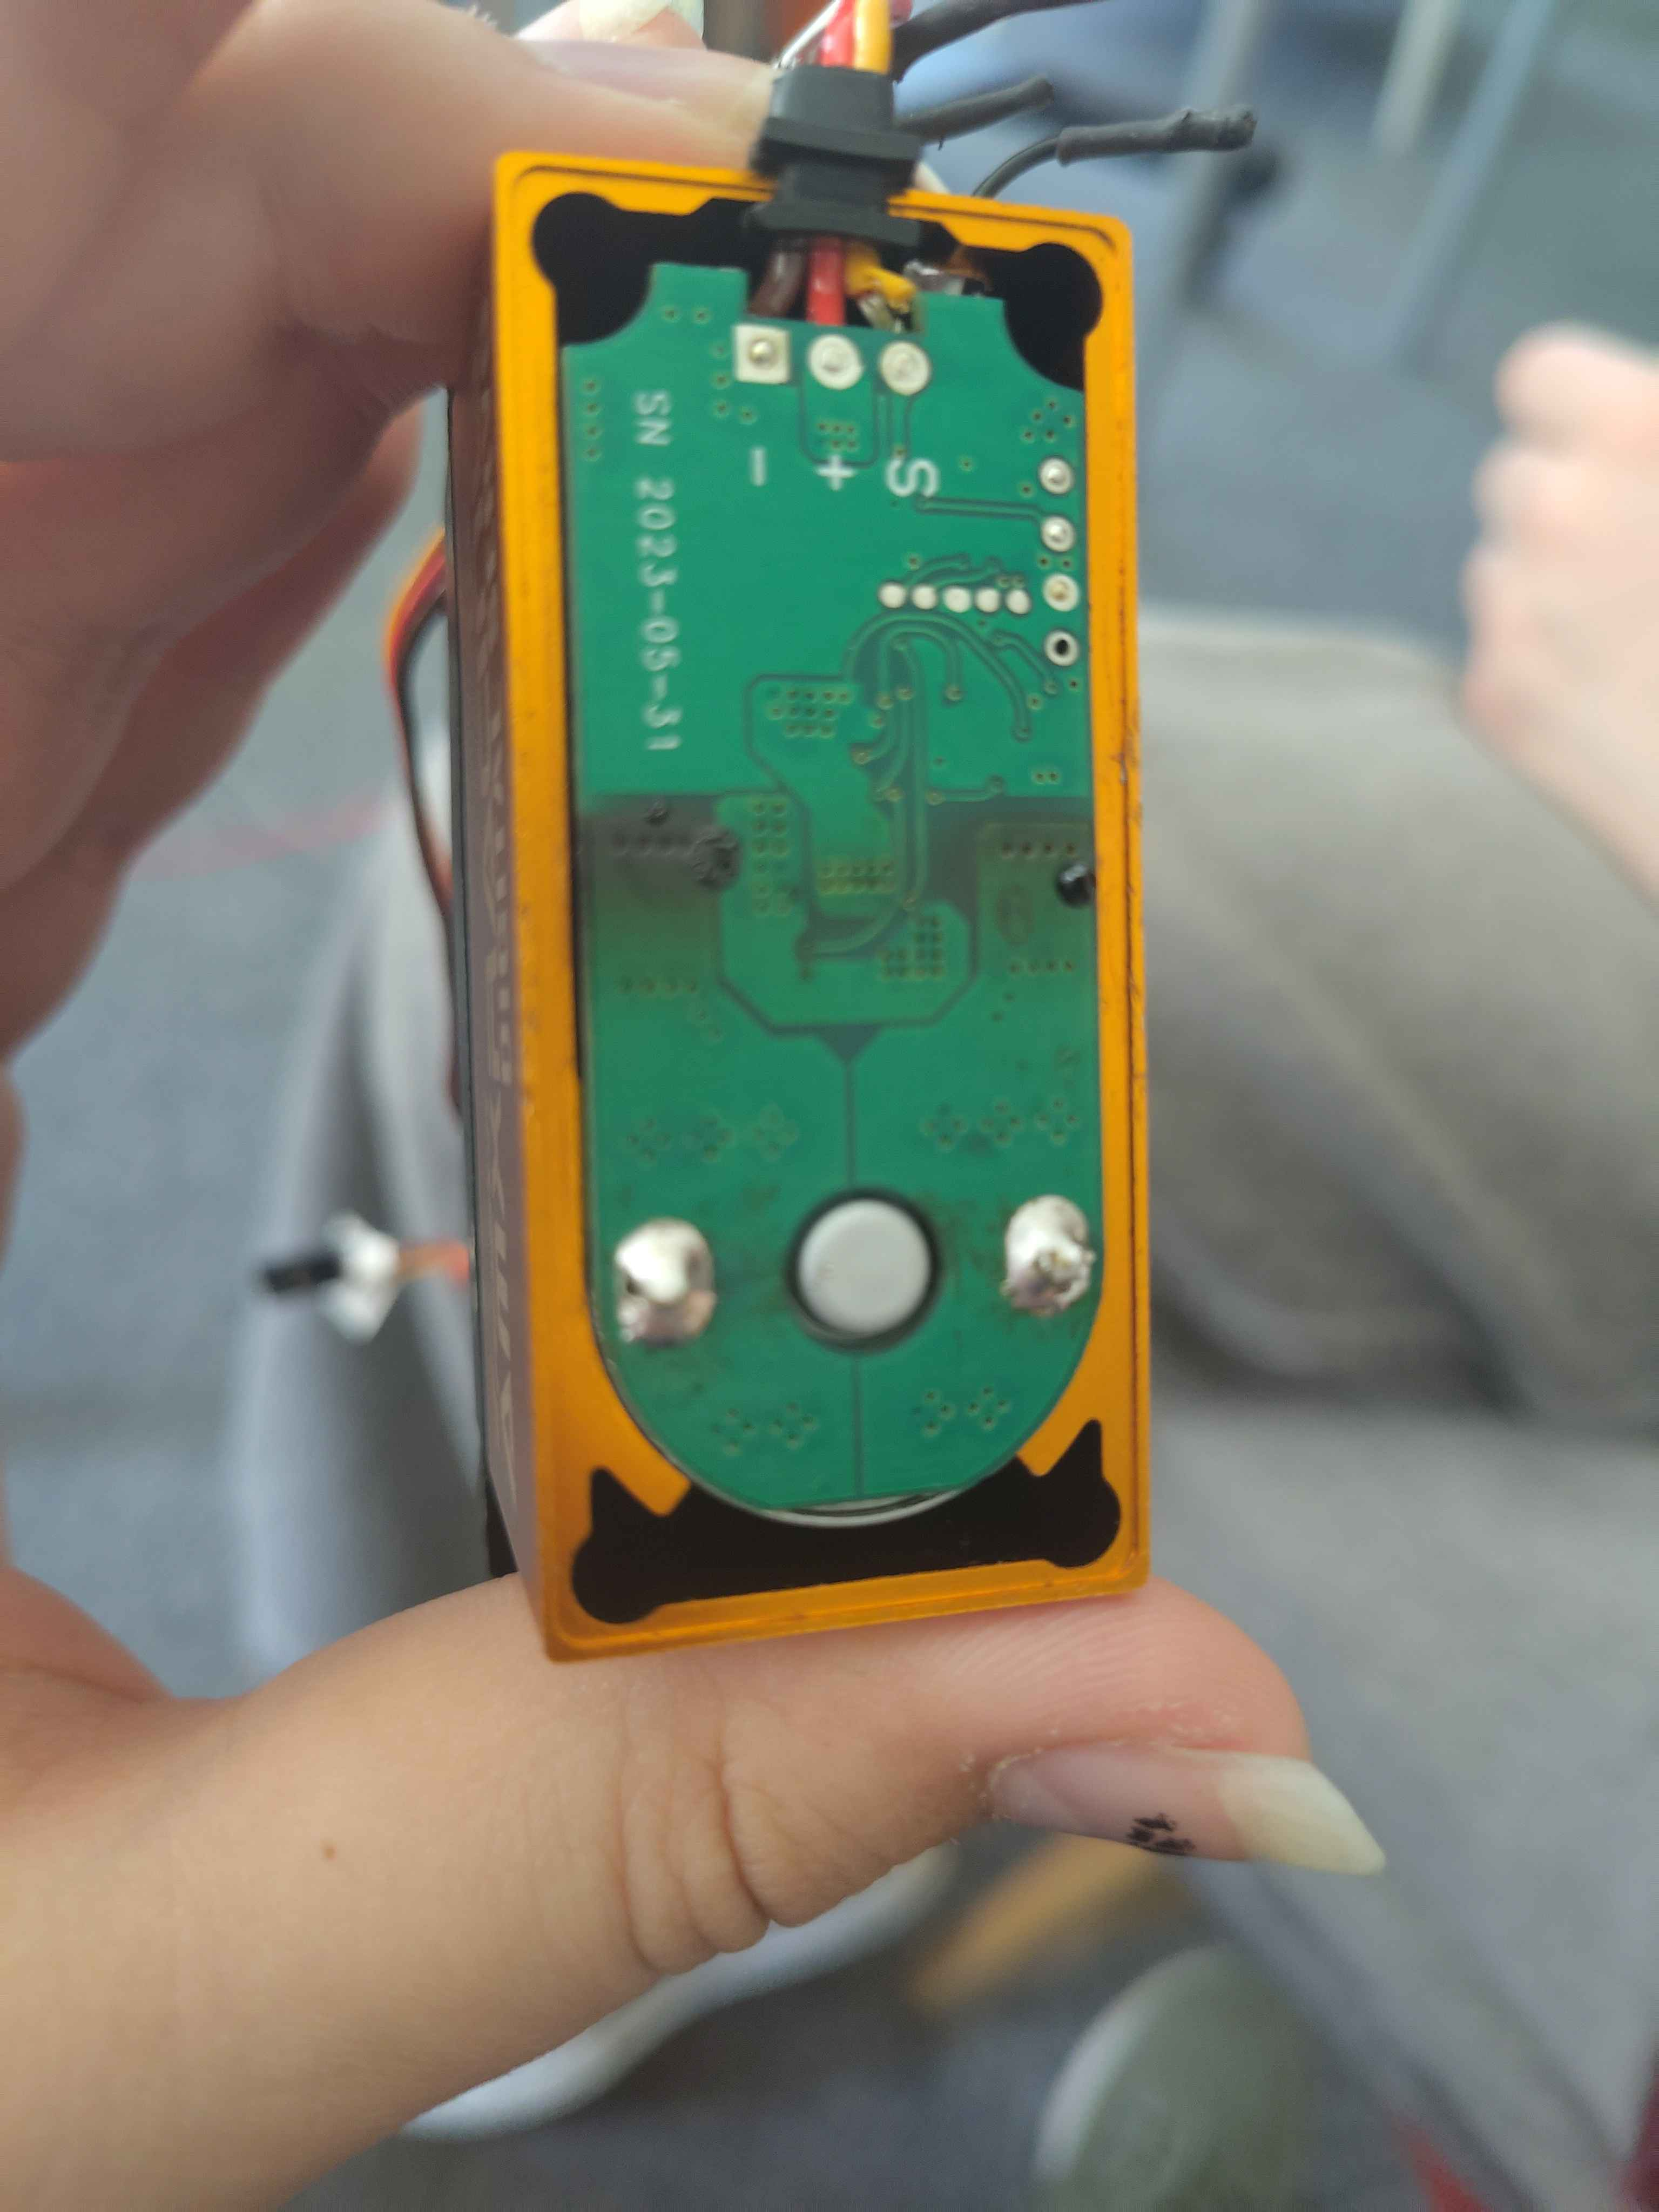
\includegraphics[width=.8\linewidth]{Media/Burnt_Motor.jpg}
    \end{subfigure}
\end{figure}

The reason for both these failures were the length of screws connecting the potentiometer being too long and digging into the worm gear.

\begin{figure}[h]
    \begin{subfigure}{.5\textwidth}
        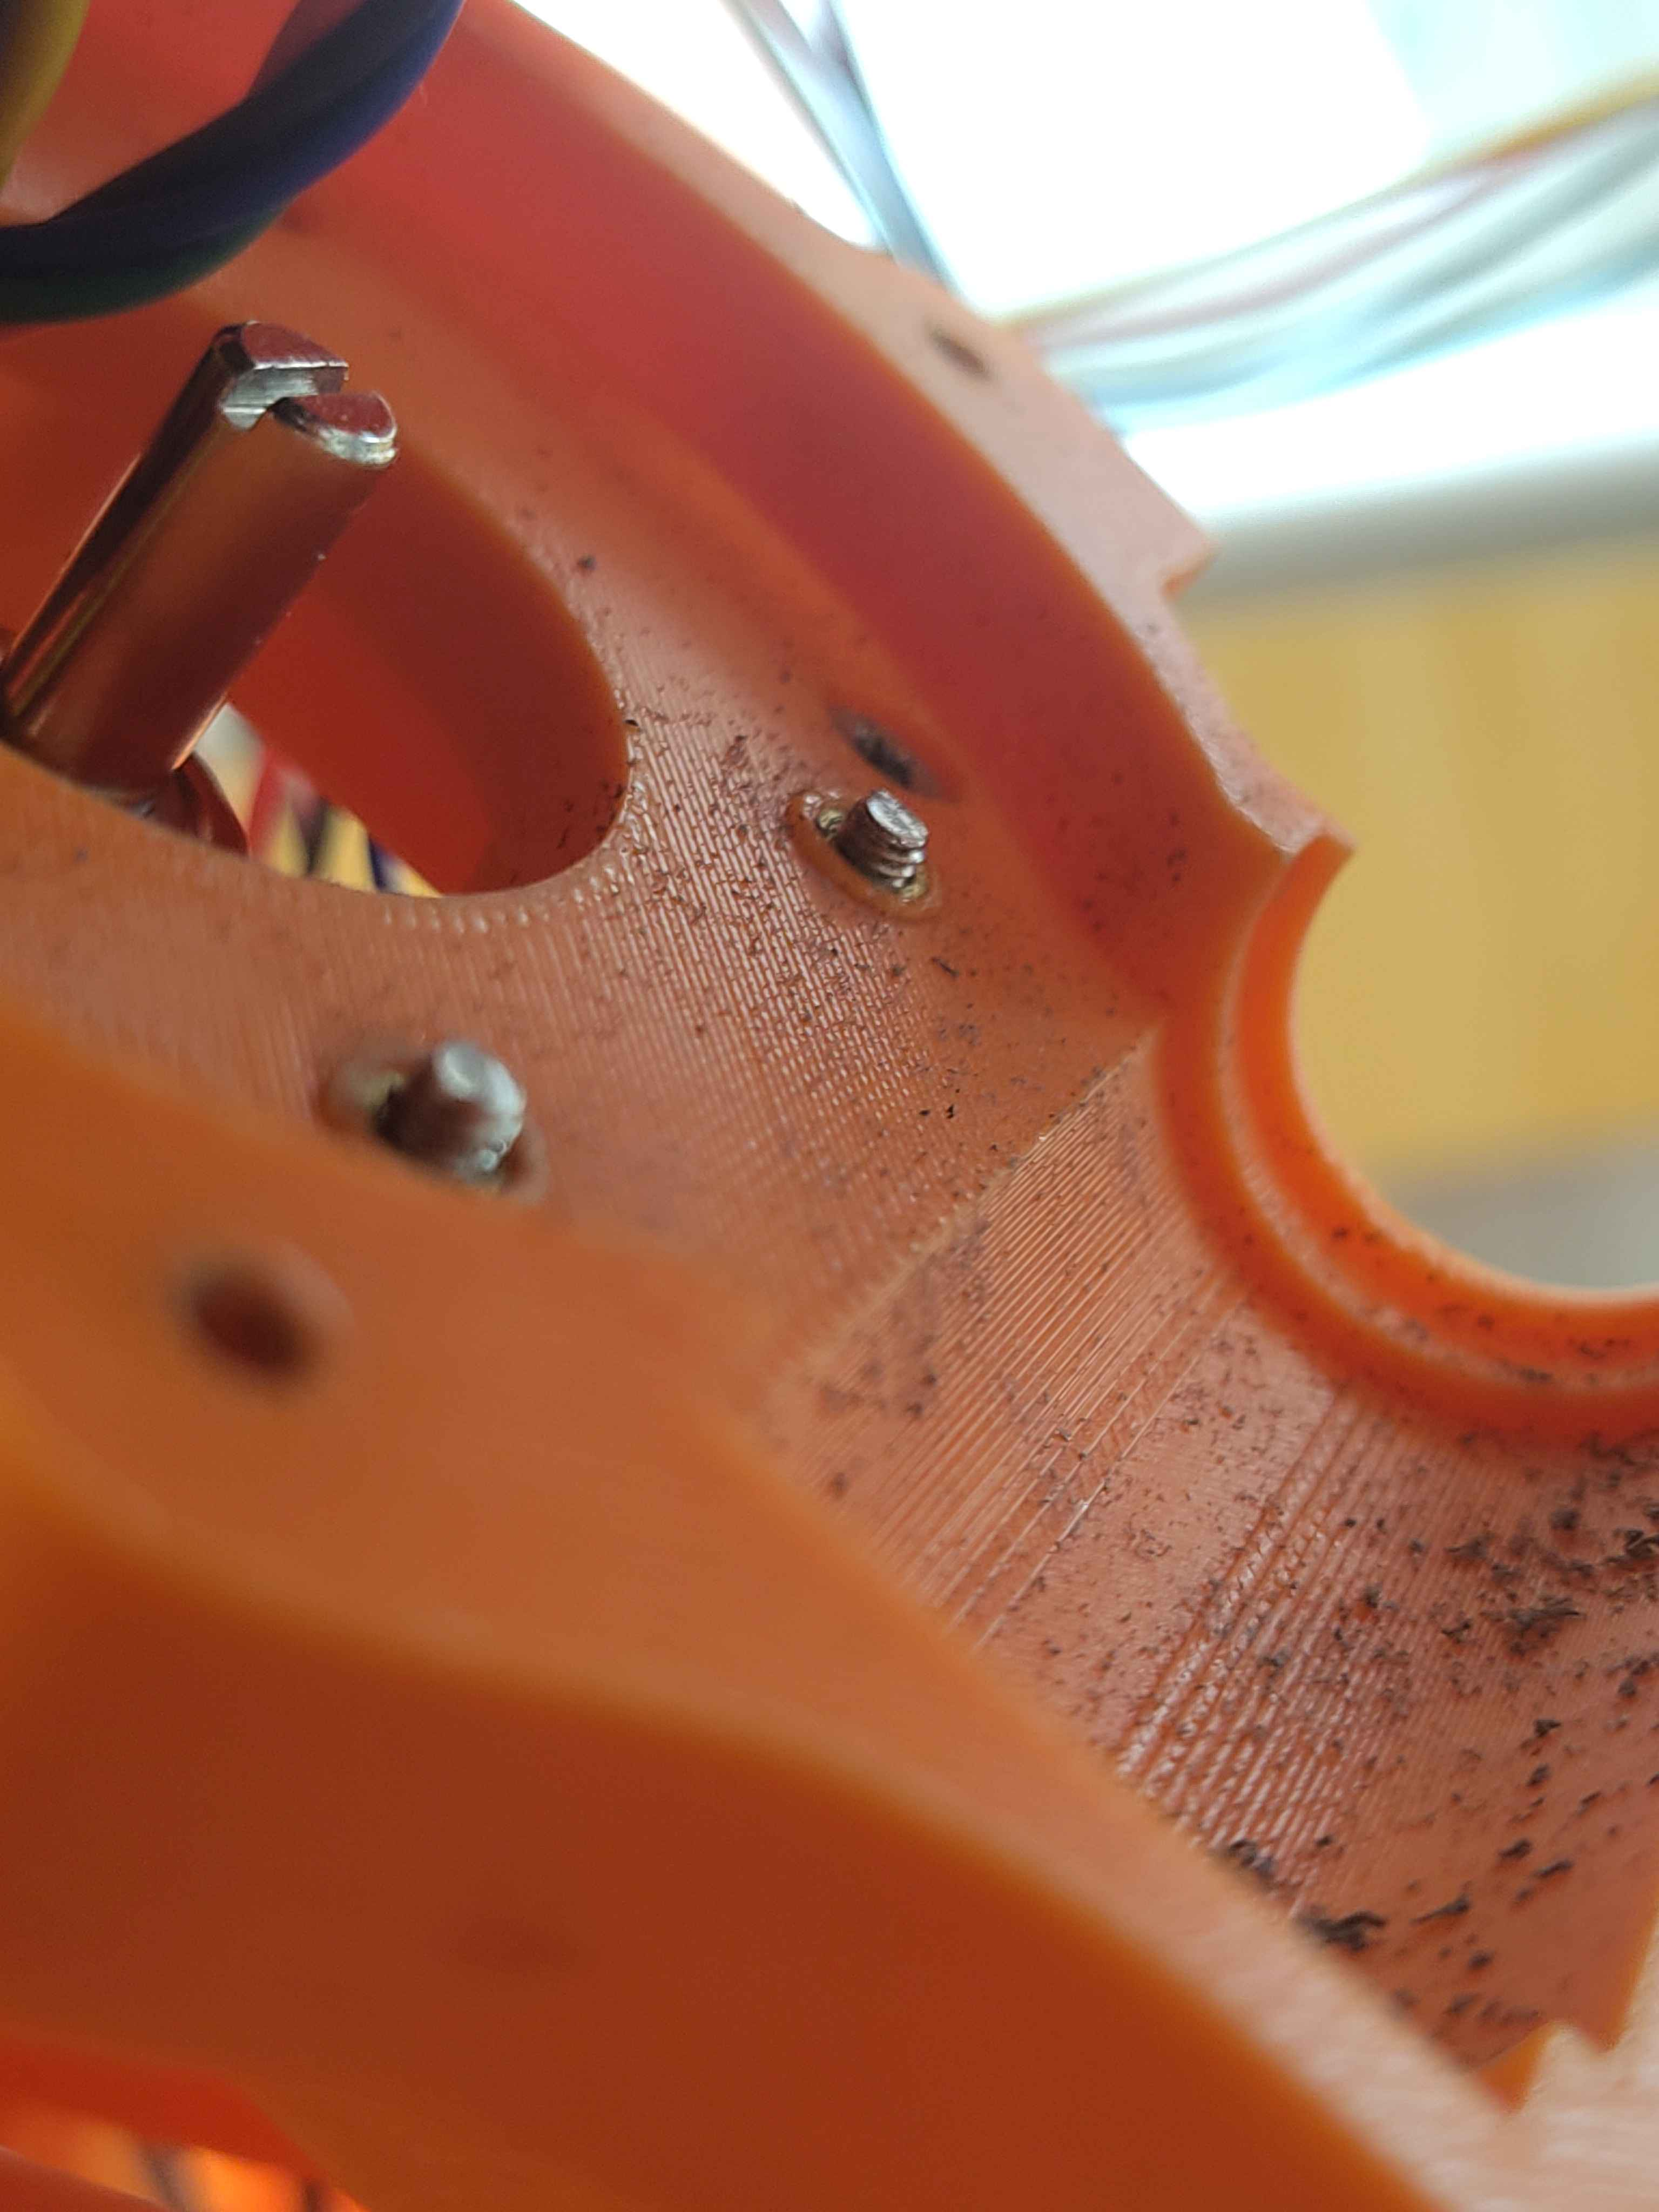
\includegraphics[width=.8\linewidth]{Media/Potentiometer_Screws.jpg}
    \end{subfigure}
    \begin{subfigure}{.5\textwidth}
        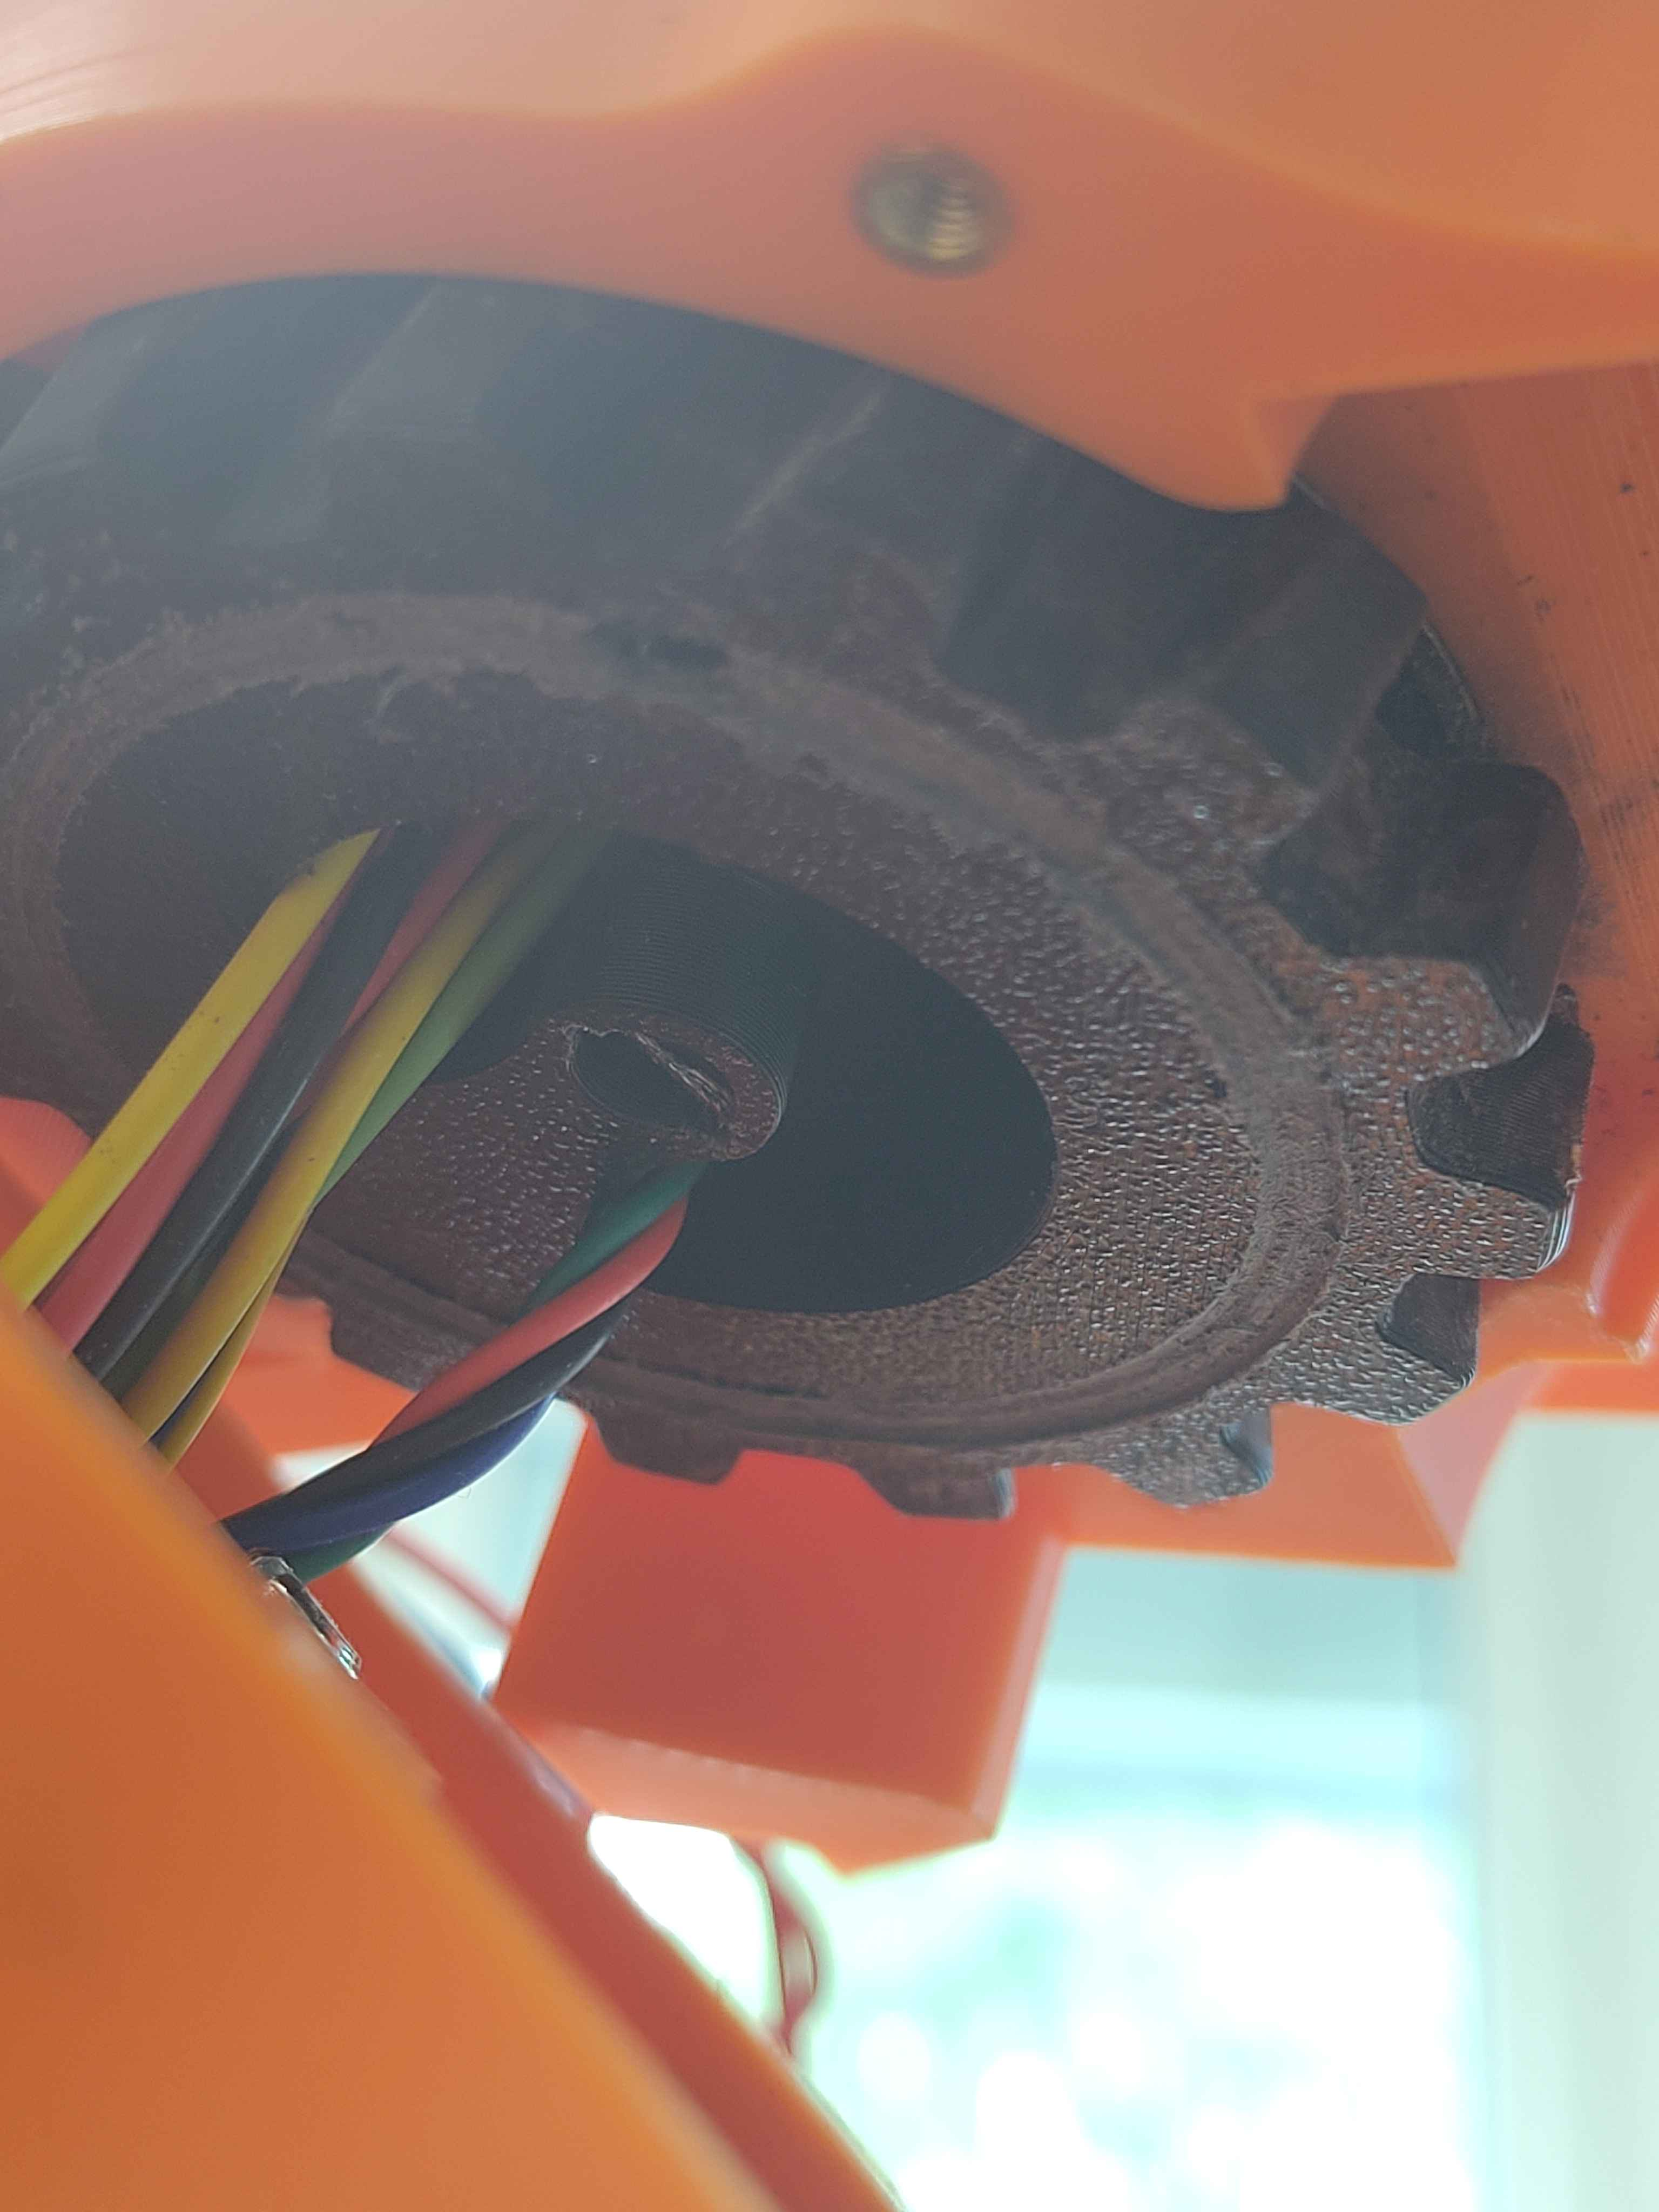
\includegraphics[width=.8\linewidth]{Media/Worm_Gear_Broken.jpg}
    \end{subfigure}
\end{figure}

This caused enough friction to require the motor to work incredibly hard until the breaking of the part gave the motor a back current strong enough to fry the MOSFETs.


The screws were exchanged for shorter ones, the gear, worm and casing were printed anew.

\subsection{Outer Bicep}

Underneath the outercasing of the bicep there is a step down circuit which was not acounted for in the original design which made the plate crack when tightened.

The new plate is thickened to enable a dugout for this part while still fitting the surounding parts. 

The skeletal board underneath ought to be extended to match this new hight to cover the dugout from view.

\subsection{Inner Bicep}

Simply made to match the outer Bicep for aesthetic reasons.

\subsection{Finger Nylon Thread}

The nylon thread connecting the ring finger was replaced. The underlying sharp edges were not addressed. 

\section{Electrical}

\subsection{Powerline Quick Disconnect}

\subsection{Shoulder Rotation Quick Disconnect}

\subsection{Upper Arm IMU Cable Connector}

\section{Software}

\end{document}